\part{Aspectos Gerais}
\chapter[Introdução]{Introdução}

\chapter{Requisitos\label{ch:requisitos}}

A Engenharia de requisitos estuda como coletar, entender, armazenar, verificar e gerenciar requisitos. Sua principal preocupação é entender e documentar quais são os requisitos reais do sistema \cite{belgamo2000}. Ela é dividida em diferentes fases: Elicitação, Análise, Especificação, Verificação e Gerenciamento.

A Elicitação é definida como o processo de  compreensão dos requisitos dos steakholders \cite{yousuf2015}, e é o primeiro estágio para a construção do entendimento sobre o problema. Para isso existem diferentes técnicas para que os requisitos sejam coletados de maneira correta e eficiente. Neste projeto foram utilizadas duas técnicas:
Questionário e Brainstorming.

A aplicação de questionários é um dos métodos de elicitação de requisitos de menor custo. Esta técnica costuma alcançar uma grande quantidade de pessoas, em menos  tempo e com baixo custo \cite{gunda2008}. Para aplicar esta técnica foi utilizada a ferramenta Google Forms, que permite o compartilhamento do questionário em diversas redes sociais. As respostas são fornecidas pela plataforma em texto, quando as questões são dissertativas, ou em gráficos, como mostra a figura a seguir.

\begin{figure}[h]
  \caption{Questionário sobre problemas da FGA}
  \centering
    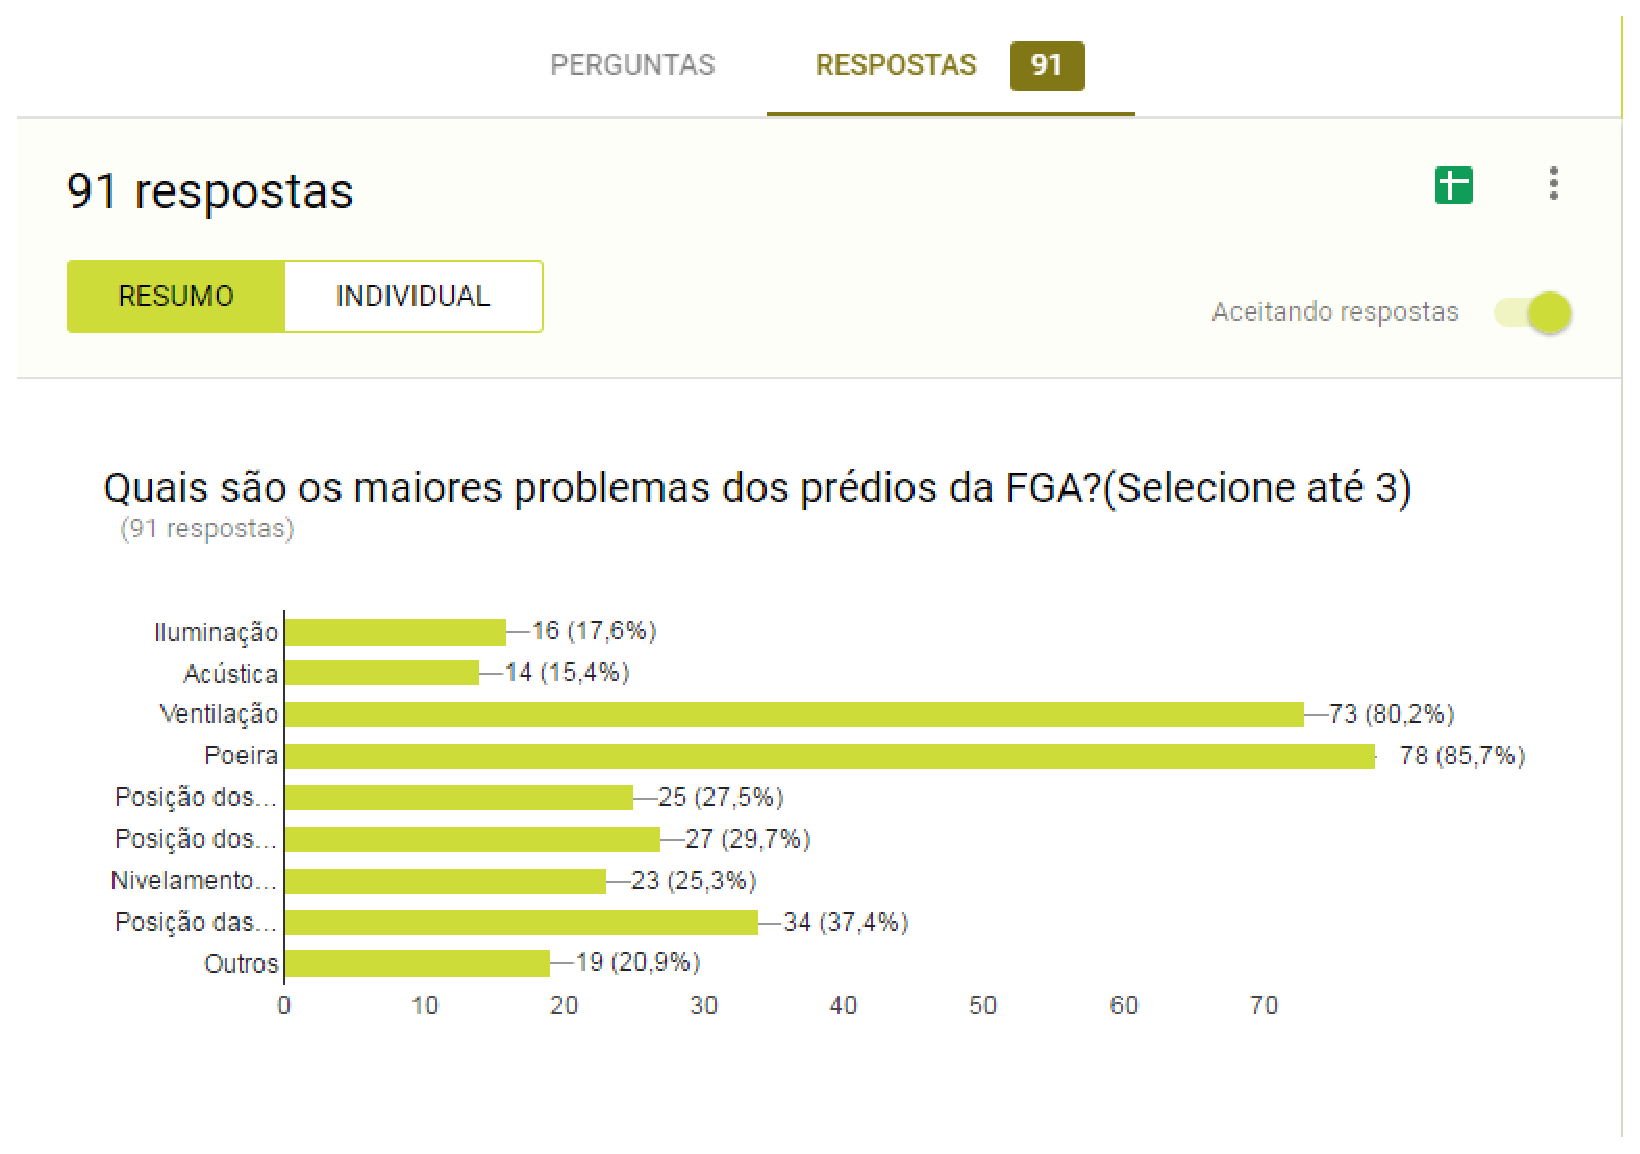
\includegraphics[width=1.0\textwidth]{figuras/pesq.eps}
\end{figure}

Brainstorming é uma técnica de grupo utilizada para criar novas ideias para o projeto e/ou encontrar soluções para um problema específico, além de possibilitar o diagnóstico de problemas em pouco tempo. São conduzidos como uma conferência reunindo de seis a dez membros, onde cada membro tem o direito de explanar suas ideias em um certo período de tempo. Esta reunião possui um mediador, que define a questão a ser discutida \cite{gunda2008}.

Esta técnica foi aplicada por meio de uma reunião com toda a equipe, onde, baseadas nos requisitos fornecidos na descrição do projeto do prédio inteligente, as ideias geradas foram anotadas em um documento editável no Google Drive. Ao longo da semana, todos os membros da equipe poderiam continuar escrevendo suas ideias no documento, que foram discutidas e priorizadas na aula seguinte, novamente com toda a equipe. Nesta reunião foi realizada a Análise dos requisitos gerados pelas técnicas de elicitação.

Estes requisitos foram documentados no Backlog do Produto, mostrado na figura ~\ref{fig:backlog}, onde os requisitos foram agrupados visando a rastreabilidade vertical, partindo de grandes blocos mais genéricos chamados Épicos, que são divididos em partes menores chamadas Features.


\chapter{Escopo}
Para a realização do projeto Prédio inteligente deve-se definir as especificações do limite que contempla o projeto, para isso foi necessário definir os requisitos e analisá-los e aplicar alguns métodos para facilitar a definição do escopo como o dos 5W e 2H representado abaixo:

1-What -O que será feito ?

2-Who- Por quem será feito ?

3-Where- Onde será feito ?

4-When-Quando será feito?

5-Why-Por que será feito?

6-How-Como será feito ?

7-How Much- Quanto custará?

    Dessa forma o escopo foi definido como sendo o Prédio Sustentável inteligente da Faculdade do Gama(FGA) e pode ser melhor observado na EAP visto que a mesma guia a equipe para o término do projeto,não incluindo geração de energia ou algum sistema tecnológico para outra parte do campus exceto o estacionamento parte fundamental do campus que ainda não foi concluída e pode ser resolvida com ideias que possuem nesse projeto , esse escopo foi decidido com base: no  alto custo financeiro para suprir toda demanda energética do campus, futuras alterações de estruturas e dimensões dos prédios já construídos e pelo tempo de entrega do projeto.Por fim,foi realizado um escopo para que futuramente a Universidade de Brasília pudesse aproveitá-lo para a construção do novo prédio trazendo assim conforto e ferramentas necessárias para todos que necessitam do mesmo para absorver conhecimento.(stakeholders).
    Outra subdivisão do nosso projeto, trata da parte de controle de acesso, que é responsável por monitorar todo o acesso de pessoas feito neste nosso prédio tecnológico dentro da FGA. Levando em conta que o nosso trabalho é feito em uma universidade federal, não podemos fechar completamente o acesso à universidade, entretanto nosso objetivo é selecionar quem terá ou não acesso a partes específicas dentro do novo prédio.

Inicialmente a ideia é restringir uma parte do estacionamento só para alunos matriculados na faculdade, e para que seja liberada a entrada, é necessário a liberação automática mediante apresentação de carteirinha, em seguida, o acesso também será restringido nas salas e laboratórios com trancas que serão acopladas nas portas, no caso de laboratórios e salas com equipamentos mais sofisticados, somente será autorizada a entrada com um professor como responsável pelo uso do ambiente, e no caso das salas simples, também haverá necessidade de um responsável, contudo, poderá ser tanto aluno, monitor ou professor. A frequência também será averiguada mediante carteirinha em um aparelho eletrônico portátil que cada professor possuirá. Essa tecnologia e modo de segurança já é utilizado em várias universidades do mundo e especialmente em algumas faculdades particulares em Brasília e por isso é uma ideia a ser implementada dentro da UnB principalmente por questão de segurança.

Na parte estrutural do projeto serão aplicados materiais inteligentes e sustentáveis para amenizar a produção de resíduos e consequentemente o impacto no meio ambiente. Além disso, serão consideradas algumas adaptações sobre o uso das salas para se possa receber o sistema de automação e também quais serão destinadas a laboratórios ou salas de aula, de acordo com as necessidades dos usuários. Por fim, haverá a alteração da posição dos elementos usados em sala para melhorar o impacto que os mesmos têm no aprendizado.

Para a produção energética foi considerada duas formas para suprir a demanda energética da FGA a primeira e principal é a geração de energia por meio de placas fotovoltaicas e a segunda sendo utilizada como reserva será por meio de um gerador movido a biodiesel.

\section{Backlog do Produto}
Conforme discutido no capítulo \ref{ch:requisitos}, o \textit{backlog} do produto foi definido com os requisitos agrupados em uma rastreabilidade vertical, seguindo do mais abstrato (ou alto nível) para o mais específico (ou baixo nível).

\begin{figure}[!h]
  \centering
  	\includegraphics[width=0.9\textwidth]{figuras/backlog.eps}
   \caption{Backlog do Produto\label{fig:backlog}}

\end{figure}

\chapter{EAP}
	A Estrutura Analítica de Projetos (EAP), é uma ferramenta visual que é feita a partir da decomposição das etapas do projeto em ordem cronológica. Ela funciona como um facilitador para a identificação de cada etapa do projeto, facilita os processos de gerenciamento e entregas bem como a estimativa de esforço, custo e duração do mesmo. Além da principal função, a definição do escopo do projeto. A EAP é representada em diagrama, começando do tópico mais geral, em seguida as principais etapas, e por fim as entregas que cada etapa necessita.

Para o projeto do Prédio Inteligente elaborou-se uma EAP para que fosse mais fácil a visualização das etapas que devem ser seguidas, além da definição do escopo do mesmo. Essa ferramenta também serve para que todos da equipe tenham acesso à modo que o projeto será desenvolvido. Sendo assim, as fases principais foram divididas em: Planejamento, Justificativa das Soluções e Viabilidade Econômica. Implicitamente estas fases representam os Pontos de Controle 1, 2 e 3 respectivamente. Consequentemente, foram definidas as entregas que devem ser feitas para cada Ponto de Controle.
 \begin{figure}[!h]
 	\centering
 	\includegraphics[keepaspectratio=true,scale=0.37]{figuras/eap.eps}
 	\caption{EAP do Projeto Prédio Inteligente}
 	\label{fig01}
 \end{figure}
